\documentclass[a4paper, 12pt]{article}

\usepackage{graphicx}
\usepackage{subcaption}
\usepackage{url}
\usepackage{rotating}
\usepackage{amsmath}
\usepackage{siunitx}

\title{Semester assignment in ElMag, problem 2\\
  \centering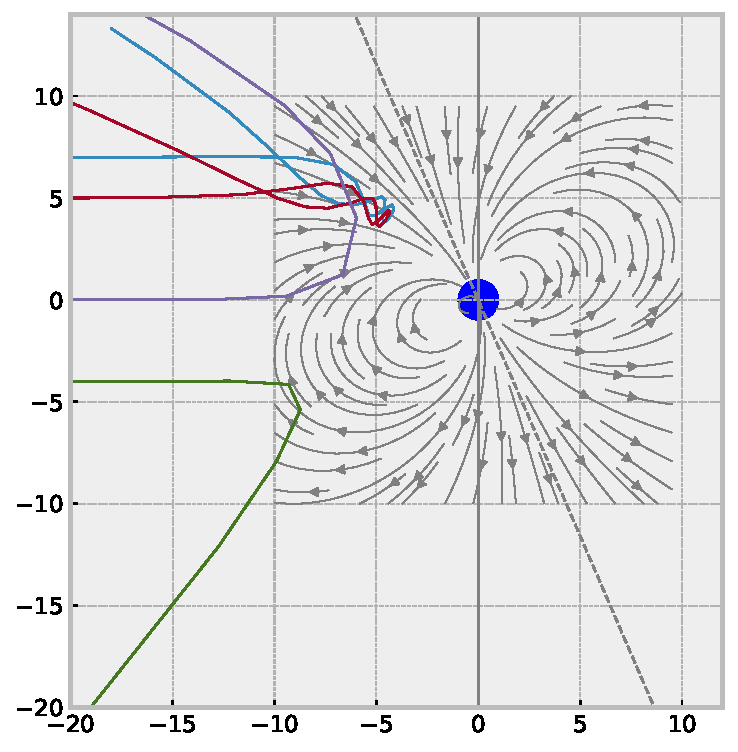
\includegraphics[width=10cm]{media/front_image}}
\author{Thorvald M. Ballestad}

\begin{document}
\maketitle
\section{Introduction}
We will model Earth's magnetic field to study the motion of charged particles from the sun.

\section{Theory}
It is here assumed that the reader knows everything in Griffiths and the problem text.

The Earth is modeled as a dipole, with dipole moment $\vec{m}$. The $\vec{B}$-field is then
\begin{equation}\label{eq:bfield}
\vec{B}(\vec{r}) = \frac{\mu_0}{4\pi}
\left[
  \frac{3\vec{r}(\vec{m}\cdot \vec{r})}{r^5} - \frac{\vec{m}}{r^3}
  \right].
\end{equation}
For Earth $m \approx \SI{8E22}{\ampere\meter\squared}$.
The mean radius of Earth is $R_j \approx \SI{6.4E6}{\meter}$ and the typical speed of a solar wind is $V_0 \approx \SI{3E5}{\meter\per\second}$.
The fields are shown in figure \ref{fig:xy_field} and figure \ref{fig:xz_field}.

\begin{figure}[h]
  \centering
  \begin{subfigure}[b]{0.47\textwidth}
    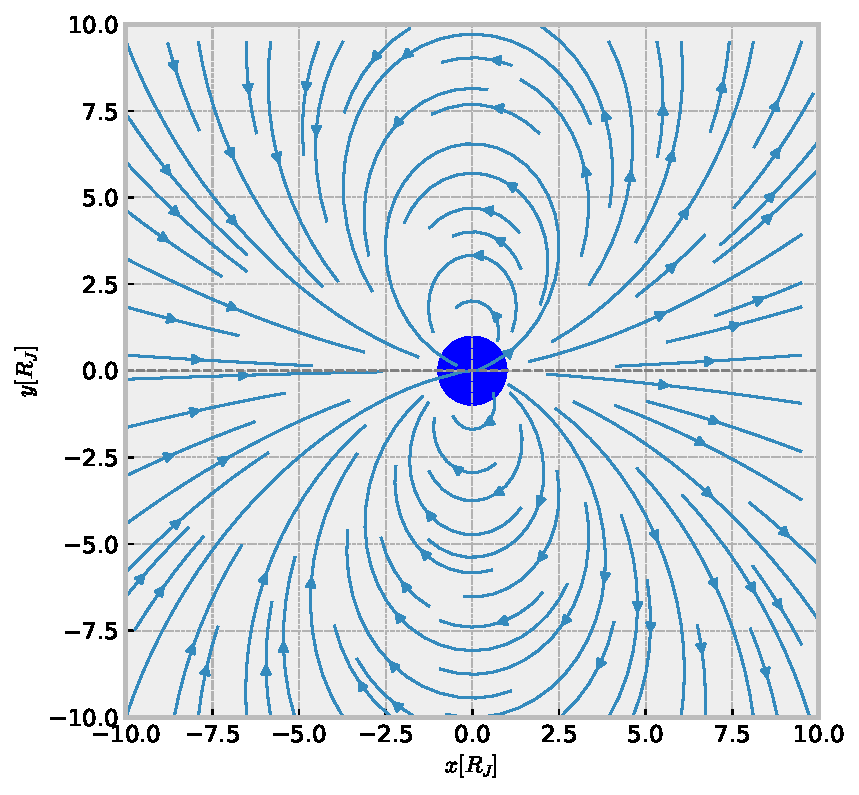
\includegraphics[width=\textwidth]{media/B_field_xy_plane}
    \caption{$\vec{B}$-field in the $xy$-plane.\label{fig:xy_field}}
  \end{subfigure}
  \begin{subfigure}[b]{0.47\textwidth}
    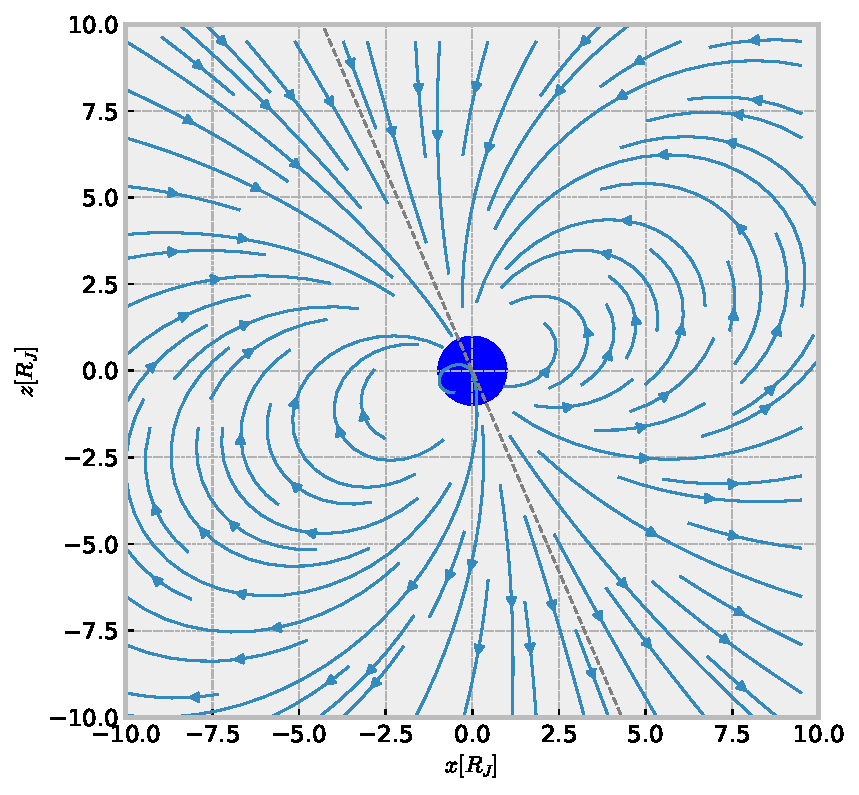
\includegraphics[width=\textwidth]{media/B_field_xz_plane}
    \caption{$\vec{B}$-field in the $xz$-plane.\label{fig:xz_field}}
  \end{subfigure}
  \caption{The $\vec{B}$-field.}
\end{figure}

The problem we wish to solve is
\begin{equation}\label{eq:problem}
  \vec{a} = \ddot{\vec{r}} = \vec{F}/M = \frac{q}{M} \vec{v}\times \vec{B},
\end{equation}
where $M$ is the mass of Earth.

\subsection{Units}
In the simulation we use dimensionless quantities.
They are related through Earth's mean readius and the typical velocity of solar winds.
Denoting our dimensionless variables with a prime, they are defined as follows.
\begin{align}
  r &\equiv r' R_j& \text{where } R_J = \SI{6.4E6}{\meter},\\
  v &\equiv v' V_0& \text{where } V_0 = \SI{2.5E5}{\meter\per\second}.
\end{align}

Thorough these definitions we have also implicitly defined the dimensionless time as
\begin{equation}
  t = t' t_0, \quad t_0 = \frac{R_j}{V_0} = \SI{26}{\second}.
\end{equation}

We can now write \eqref{eq:bfield} as
\begin{equation}
  \vec{B}(\hat{r}) = B_0
  \left[
    \frac{3\hat{r}(\hat{m}\cdot \hat{r}) - \hat{m}}{r'^3}
    \right],
\end{equation}
where $B_0 = \frac{\mu_0 m}{4\pi R_J^3}$.
We can now express \eqref{eq:problem} dimensionless as
\begin{equation}
  \ddot{\vec{r}'} = \frac{q V_0 B_0}{M R_J} \vec{v}' \times \vec{B}' = B_0' \vec{v}' \times \vec{B}',
\end{equation}
where $\vec{B}' = \vec{B}/B_0$.
Lastly, converting to unitless time, the final expression becomes
\begin{equation}
  \frac{\mathrm{d}^2\vec{r}'}{\mathrm{d}t'^2} = t_0^2 B_0' \vec{v}' \times \vec{B}'.
\end{equation}
By construction, $t_0^2 B_0' \approx \num{6E4}$ is dimensionless.

\subsection{ODE}
Our equation to solve is a second order differential equation.
We use scipy's integration module to solve it, using the RK45 method.

\section{Results}
\begin{figure}[h]
  \centering
  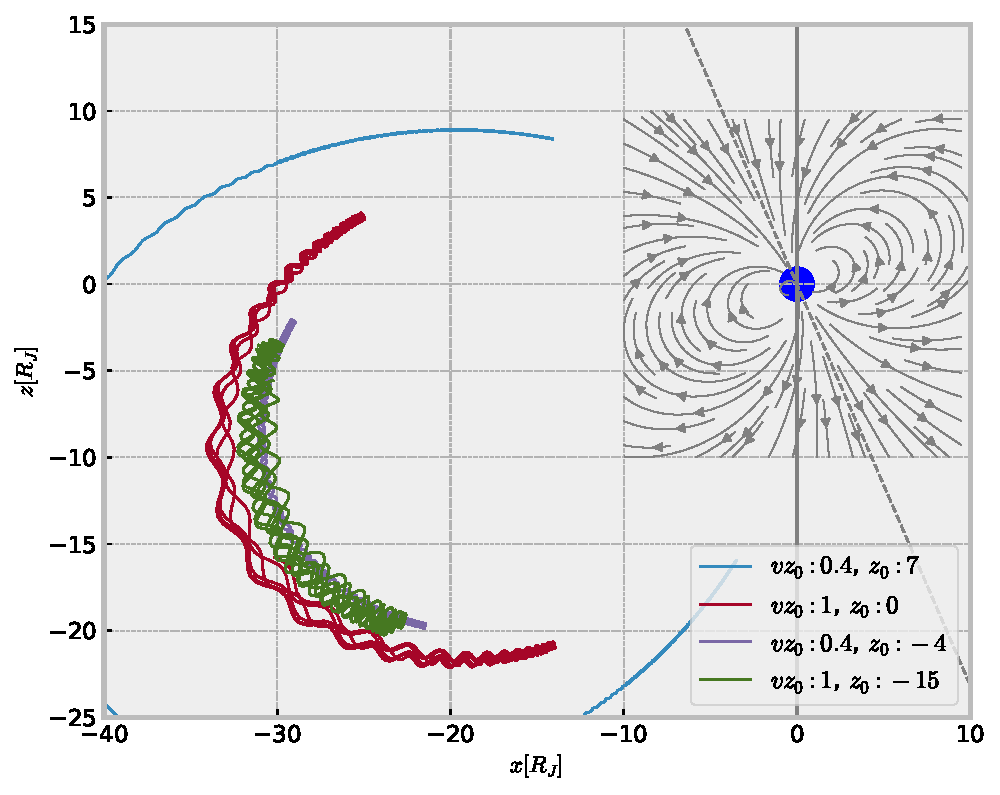
\includegraphics[width=\textwidth]{media/trajectory_xz_plane}
  \caption{Trajectory in the $xz$-plane.\label{fig:trajectory_xz}}
\end{figure}

\begin{figure}[h]
  \centering
  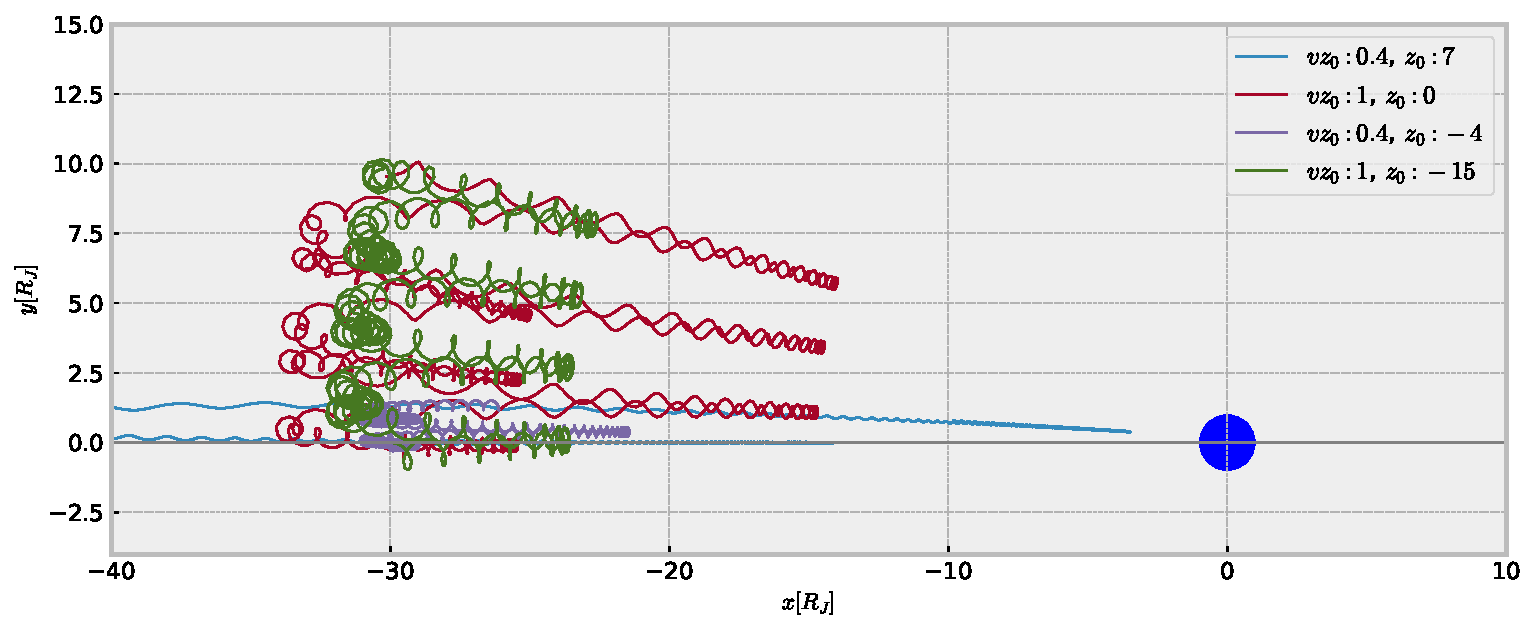
\includegraphics[width=\textwidth]{media/trajectory_xy_plane}
  \caption{Trajectory in the $xy$-plane.\label{fig:trajectory_xy}}
\end{figure}
We see from figure \ref{fig:trajectory_xz} and figure \ref{fig:trajectory_xy} that the particles are locked in a path following the magnetic field lines -- a magnetic mirror.
Different initial conditions affect the radius and length of the arc path, and also the inital direction of the path.
Particles starting below the ecliptic plane, for example the particle with $z_0 = -15$ in figure \ref{fig:trajectory_xz}, will initially move along the path going in negative $z$-direction, while particles starting above the ecliptic plane moves in positive $z$-direction.
They are both, however, locked into the same type of arc path.
For particles with paths of the same radius, the arc of particles with higher kinetic energy is longer.
That is, their extremum points are closer to the Earth.
Particles with larger radii have extremum points closer towards Earth than particles with smaller radii and the same kinetic energy.

\subsection{Dependence on field strength}
The trajectories depend on the strength of the magnetic field.
Only when the field is sufficiently strong, do we get the magnetic mirror effect.
In figure \ref{fig:trajectory_xz_weak} trajectories for particles with the same inital conditions as in figure \ref{fig:trajectroy_xz} is shown, but with a weaker magnetic field.
Here the magnetic field is set to $\num{2E3}$, as opposed to $\num{6E4}$ that we found in the previous discussion.
There are magnetic mirror-tendencies, but the particles are reflected rather that trapped.\\

\begin{figure}[h]
  \centering
  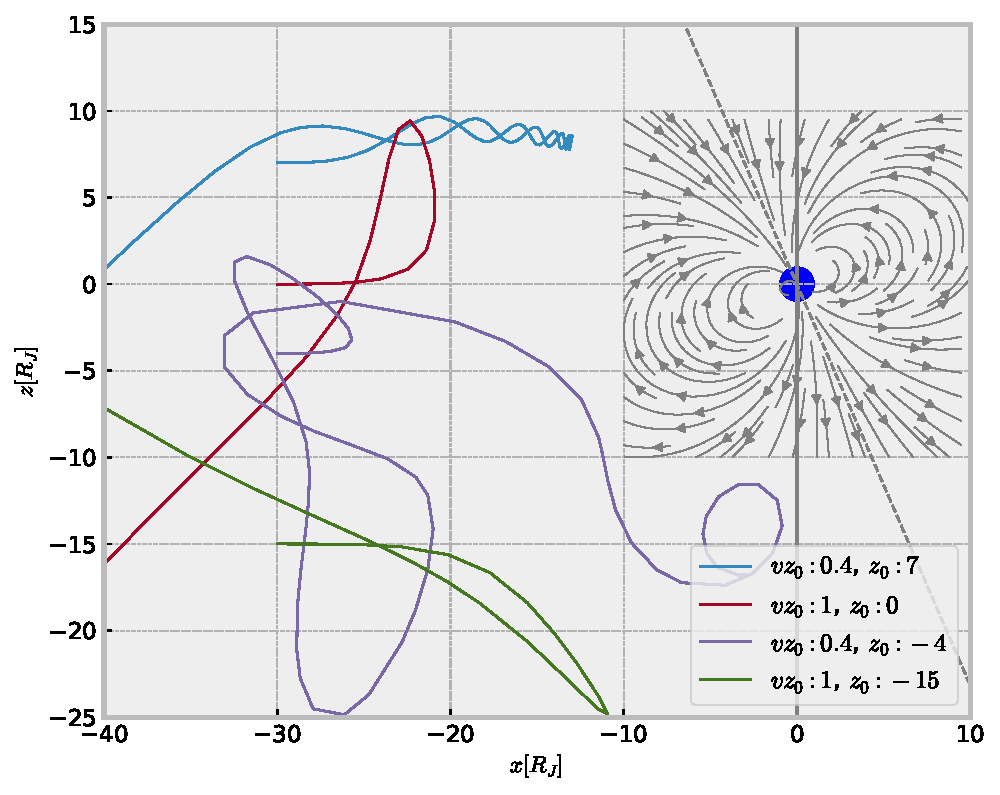
\includegraphics[width=\textwidth]{media/trajectory_xz_plane_weak}
  \caption{Trajectory in the $xz$-plane with weaker field strength.\label{fig:trajectory_xz_weak}}
\end{figure}

We use energy conservation as a check for numerical validity.
As written in the problem text magnetic force does no work, and thus the energy should remain constant.
From figure \ref{fig:energy} we see that the relative error in the energy does not exceed 0.9\%, which is considered sufficient in this case.

\begin{figure}[h]
  \centering
  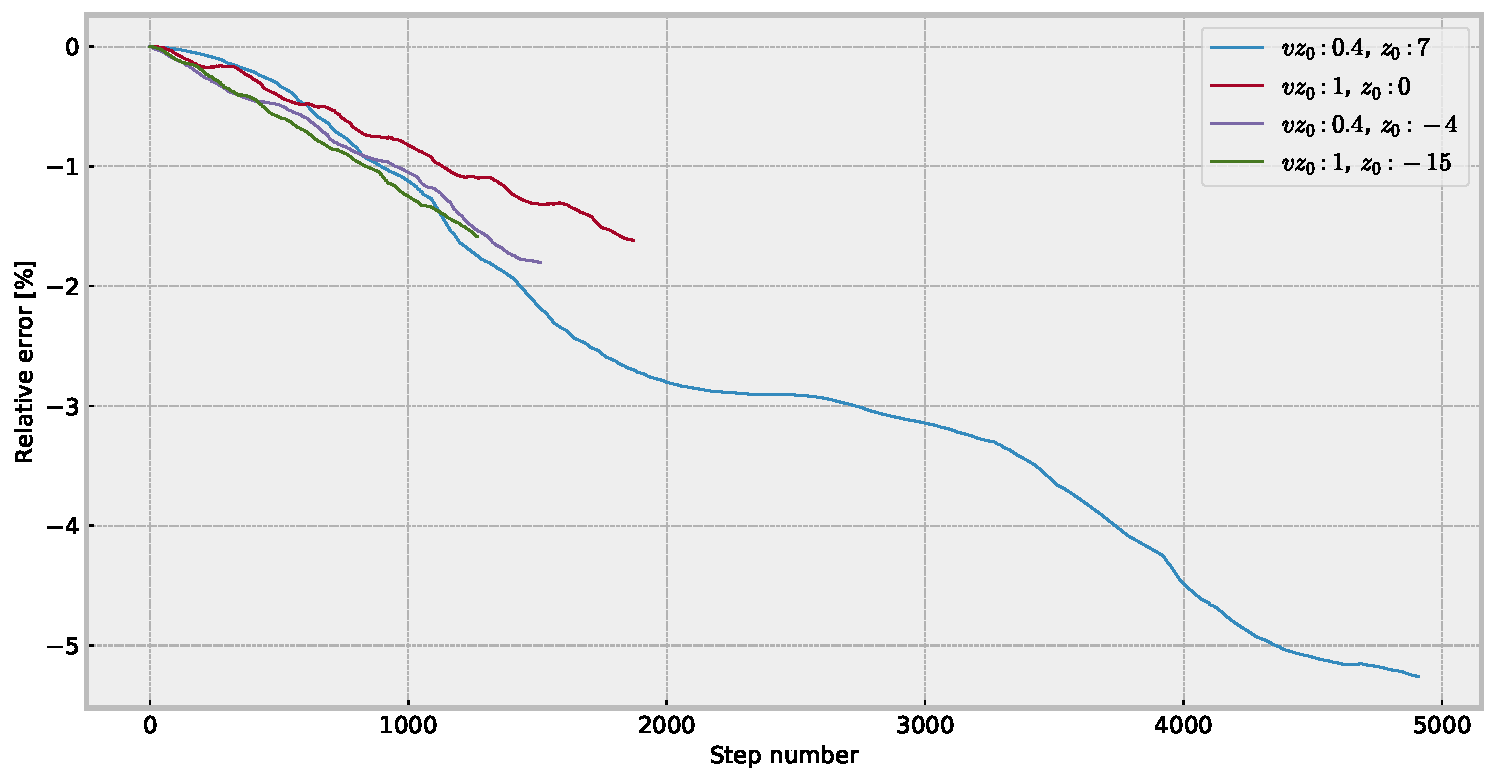
\includegraphics[width=0.75\textwidth]{media/energy}
  \caption{The energy as a function of time. Used for numeric validation.\label{fig:energy}}
\end{figure}

\section{Discussion/conclusion}
Life on Earth is completely dependent on the shielding that Earth's magnetic field provides.\cite{wiki-mag}
This very simple model is abel to capture this effect!\\

Without more experimental data, it is hard to say to what degree this model is correct.
However, this experiment shows that it is possible to trap particles in helical trajectories, and that such paths tends towards the poles. The polar lights could be attributet partly to this effect.

\begin{thebibliography}{9}
\bibitem{wiki-mag}
  Earth's magnetic field,
  \url{https://en.wikipedia.org/wiki/Earth\%27s_magnetic_field},
  Retrieved: Feb 21st 2020.
\end{thebibliography}
\end{document}
